\documentclass{article}

\usepackage{amsmath, amsthm, amssymb, amsfonts}
\usepackage{thmtools}
\usepackage{graphicx}
\usepackage{setspace}
\usepackage{geometry}
\usepackage{float}
\usepackage{hyperref}
\usepackage[utf8]{inputenc}
\usepackage[serbian]{babel}
\usepackage{framed}
\usepackage[dvipsnames]{xcolor}
\usepackage{tcolorbox}

\colorlet{LightGray}{White!90!Periwinkle}
\colorlet{LightOrange}{Orange!15}
\colorlet{LightGreen}{Green!15}

\newcommand{\HRule}[1]{\rule{\linewidth}{#1}}

% Za bolje razlomnke?
\newcommand\ddfrac[2]{\frac{\displaystyle #1}{\displaystyle #2}}
% Alias radi lakseg pisanja
\newcommand{\laj}{\sqrt{\lambda_J\lambda_A}}

\declaretheoremstyle[name=Theorem,]{thmsty}
\declaretheorem[style=thmsty,numberwithin=section]{theorem}
\tcolorboxenvironment{theorem}{colback=LightGray}

\declaretheoremstyle[name=Proposition,]{prosty}
\declaretheorem[style=prosty,numberlike=theorem]{proposition}
\tcolorboxenvironment{proposition}{colback=LightOrange}

\declaretheoremstyle[name=Principle,]{prcpsty}
\declaretheorem[style=prcpsty,numberlike=theorem]{principle}
\tcolorboxenvironment{principle}{colback=LightGreen}

\setstretch{1.2}
\geometry{
    textheight=9in,
    textwidth=5.5in,
    top=1in,
    headheight=12pt,
    headsep=25pt,
    footskip=30pt
}

% ------------------------------------------------------------------------------

\setlength\parindent{0pt}

\title{ \normalsize \textsc{}
		\\ [2.0cm]
    \HRule{1.5pt} \\ [0.5cm]
		\LARGE \textbf{{Bitka za Ivo Džimu}}
    \HRule{1.5pt} \\[5pt] 
        \textit{Osnove matematičkog modeliranja} \\
        {- Seminarski rad -}\vspace*{9\baselineskip}
		}
\date{Matematički fakultet \\ Beograd \\ maj 2023.}
\author{\textbf{Autori:} \\[5pt]
    \Large{Radovan Božić \qquad Marija Škorić \qquad Danilo Matić} \\ \\
  \textit{Profesor: Zorica Dražić}}


\begin{document}

% ------------------------------------------------------------------------------
% Cover Page and ToC
% ------------------------------------------------------------------------------

\maketitle
\thispagestyle{empty}
\newpage

\tableofcontents
\pagenumbering{arabic}
\newpage

% ------------------------------------------------------------------------------

\section{Uvod}

%\hspace{\parindent}
\hspace*{5mm}
Važna bitka u II svetskom ratu se odvijala na ostrvu Ivo Džima. Tamo je 21500
japanskih vojnika dočekalo iskrcavanje 54000 Amerikanaca.  Stope efikasnosti dve
vojske su procenjene na \(\lambda_A = 0.0106\) i \(\lambda_J = 0.0544\) po danu
borbe za američku i japansku vojsku, respektivno. Razvijamo matematički model
bitke baziran na sistemu diferencijalnih jednačina.



\section{Model}

\hspace*{5mm}
Baziramo model na Lančesterovom zakonu bitke naoružanih vojski (Lanchester’s
Square Law)~\cite{wiki}. Označićemo sa \(A\) --- Amerikance, a sa \(J\) --- Japance.

\begin{equation}\label{pocetna_A}
\frac{dA}{dt} = - \lambda_{J}J
\end{equation}

\begin{equation}\label{pocetna_J}
\frac{dJ}{dt} = - \lambda_{A}A
\end{equation}


Ovaj sistem diferencijalnih jednačina možemo rešiti deljenjem ove dve jednačine,
i iz toga dobijamo:

\[
  \frac{\displaystyle \frac{\displaystyle dA}{\displaystyle dt}}{\displaystyle  \frac{\displaystyle dJ}{\displaystyle dt} } = \frac{\displaystyle dA}{\displaystyle dJ}
\]

\[
  \frac{\displaystyle dA}{\displaystyle dJ} = \frac{\displaystyle \lambda_{J}J}{\displaystyle \lambda_{A}A}
\]

\begin{equation}\label{za_integ}
  \lambda_{A}A\,dA = \lambda_{J}J\,dJ
\end{equation}

integralimo jednačinu (\ref{za_integ}):

\[
  \lambda_{A}\int{} A\,dA = \lambda_{J} \int{} J\,dJ
\]

\[
  \lambda_{A} \frac{\displaystyle A^2}{\displaystyle 2} + \underbrace{c\lambda_{A}}_{c_1}
  = \lambda_{J} \frac{J^2}{2} + \underbrace{c\lambda_{J}}_{c_2}
\]

\begin{equation}\label{jedn1}
  \lambda_{A} \frac{A^2}{2} - \lambda_{J} \frac{J^2}{2} = c_2 - c_1 = c
\end{equation}

Za trenutak \(t = t_0 = 0\), sledi \(A(t_0) = A_0\) i \(J(t_0) = J_0\). Menjamo
u jednačini (\ref{jedn1}) i dobijamo:

\begin{equation}\label{jedn2}
  \lambda_{A}\frac{A_{0}^2}{2} - \lambda_{J}\frac{J_{0}^2}{2} = c
\end{equation}

Izjednačavamo jednačine (\ref{jedn1}) i (\ref{jedn2}):

\[
  \lambda_{A}\frac{A^2}{2} - \lambda_{J}\frac{J^2}{2} =
\lambda_{A}\frac{A_{0}^2}{2} - \lambda_{J}\frac{J_{0}^2}{2}
\]

Sređivanjem dobijamo:
\begin{equation}\label{izjednacena}
  \lambda_{A}A^2 - \lambda_{A}A_{0}^2 = \lambda_{J}J^2 - \lambda_{J}J_{0}^2
\end{equation}

Bitka traje dok jedna od strana ne izgubi sve vojnike. Ako uzmemo da je broj
Japanca na kraju jednak nuli (\(J = 0\)), sređivanjem jednačine
(\ref{izjednacena}) se dobija da je broj Američkih vojnika na kraju bitke
jednak:

\[
  \lambda_{A}A^2 - \lambda_{A}A_{0}^2 = -\lambda_{J}J_{0}^2,
\]

\begin{equation}\label{za_uslov}
  \lambda_{A}A^2 = \lambda_{A}A_0^2 - \lambda_{J}J_0^2
\end{equation}

\[
  A^2 = A_{0}^2 - \frac{\lambda_J}{\lambda_A}J_0^2,
\]

\begin{equation}\label{brojAmeri}
  A = \sqrt{A_{0}^2 - \frac{\lambda_J}{\lambda_A}J_0^2}
\end{equation}

Iz jednačine (\ref{za_uslov}) sledi uslov: 

\begin{equation}\label{uslovAmeri}
\lambda_{A}A_0^2 \geq \lambda_{J}J_0^2.
\end{equation}

Analogno se izvodi kad je broj Amerikanaca na kraju nula (\(A = 0\)):

\[
  J = \sqrt{J_0^2 - \frac{\lambda_A}{\lambda_J}A_0^2},
\]

\begin{equation}\label{uslovJapanci}
\lambda_{A}A_0^2 \leq \lambda_{J}J_0^2
\end{equation}

Uslove (\ref{uslovAmeri}) i (\ref{uslovJapanci}) mozemo da koristimo kako bi na
početku videli koja je vojska snažnija~\cite{lanchRad}.

$\newline$

\hspace{5mm}
Početni sistem jednačina (\ref{pocetna_A}) i (\ref{pocetna_J}) možemo rešiti i
na sledeći način, difereciramo jednačinu (\ref{pocetna_A}) po \(t\):

\[
  A'' = -\lambda_{J}J'
\]

Izrazimo \(J'\) preko (\ref{pocetna_J}):

\[
  A'' = -\lambda_{J}(-\lambda_{A}A) = \lambda_{A}\lambda_{J}A
\]

\[
  A'' - \lambda_A\lambda_J A = 0
\]

Dobili smo linearnu diferencijalnu jednačinu drugog reda sa konstantnim
koeficijentima.  Nju rešavamo metodom karakterističnih funkcija: \(a^2 -
\lambda_A\lambda_J = 0\), i dobijamo da je:

\[
  a_{1,2} = \pm \laj
\]

Kako su \(a_1\) i \(a_2\) realna i različita rešenja, onda je

\begin{equation}\label{amerSaKoef}
  A(t) = c_{1}e^{t\laj} + c_2 e^{-t \laj} \ 
\end{equation}

Kada gornju jednačinu diferenciramo po \(t\), dobijamo

\begin{equation}\label{amerIzvod}
  A'(t) = c_1 \laj e^{t \laj} - c_2 \laj e^{-t \laj}
\end{equation}

Jednačine (\ref{amerSaKoef}) i (\ref{amerIzvod}) čine sistem preko koga mozemo
da dobijemo koeficijente \(c_1\) i \(c_2\). 

Za \(t = 0\), imamo  \(A(0) = A_0\) i
\(A'(0) = -\lambda_{J}J_0\), pa važi:

\[
  A_0 = c_1 + c_2
\]

\[
  -\lambda_{J}J_0 = c_1 \laj - c_2 \laj
\]

Pomnožimo prvu jednačinu sa \( \laj \) i dodamo je
drugoj kako bi dobili koef \( c_1 \):

\[
  A_0 \laj - \lambda_{J}J_0 = 2 c_1 \laj
\]

\[
  c_1 = \frac{A_0 \laj - \lambda_J J_0}{2\laj }
\]

Zamenom \(c_1\) u prvu jednačinu dobija se \(c_2\):

\[
  c_2 = \frac{A_0 \laj + \lambda_J J_0}{2\laj }
\]

Zamenom u jednačinu (\ref{amerSaKoef}) dobijamo izvedeno \(A(t)\):

\begin{equation}\label{ameri_cela}
  A(t) = \frac{A_0 \laj - \lambda_J J_0}{2 \laj } e^{t \laj } + \frac{A_0 \laj +
\lambda_J J_0}{2 \laj } e^{-t \laj}
\end{equation}
\\
Analognim izvođjenjem se dobija \(J(t)\):

\begin{equation}\label{japanci_cela}
  J(t) = c_1 e^{t \laj} + c_2 e^{-t \laj}
\end{equation}

\[
 c_1 = \frac{J_0 \laj- \lambda_A A_0}{2\laj},\ 
 c_2 = \frac{J_0 \laj+ \lambda_A A_0}{2 \laj}
\]


\newpage

\subsection{Bitka do istrebljenja}

\vspace{5mm}
\begin{quote}
\textbf{Zadatak 1:}
Koliko je dugo trajala bitka do istrebljenja jednog od
učesnika? Koliko je preostalo vojnika na pobedničkoj
strani?
\end{quote}


\hspace{5mm}
Zamenom konkretnih vrednosti u \(\lambda_{A}A_0^2\) i u \(\lambda_{J}J_0^2\)
dobijamo da je \(\lambda_{A}A_0^2 \geq \lambda_{J}J_0^2\). Odatle sledi da ce
Japanci izgubiti bitku.
Kako je \(J(t) = 0\) mozemo da izrazimo \(t\) koristeci jednačinu
(\ref{japanci_cela}).

\[
  0 = c_1 e^{t \laj} + c_2 e^{-t \laj}
\]

\[
  -c_1 e^{t \laj} = c_2 e^{-t \laj}
\]

Logaritmujemo celu jednačinu i posle malo sređivanja dobijamo:

\[
  ln(-c_1) + t\laj= ln(c_2) - t\laj
\]

\[
  t = \frac{ln(c_2) - ln(-c_1)}{2\laj}, 
\]

Zamenom konkretnih vrednosti računamo koeficijente \(c_1\) i \(c_2\) i dobijamo da je vreme trajanja bitke \(t = 61.778 \approx 62\) dana.
Broj američkih vojnika mozemo da izračunamo iz jednačine (\ref{brojAmeri}): 

\[
  A = \sqrt{A_{0}^2 - \frac{\lambda_J}{\lambda_A}J_0^2},
\]

gde dobijamo da je \(A =23 317.335 \approx 23 317\) vojnika.


\begin{figure}[htbp]
    \center
    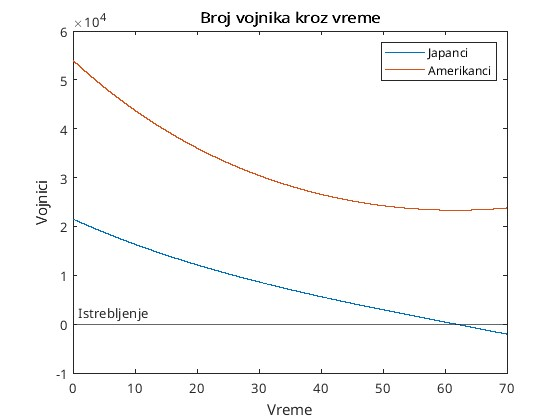
\includegraphics[scale=0.6]{img/bitka.jpg}
\end{figure}

\subsection{Pojačanje posle 30 dana}

\vspace{2mm}
\begin{quote}
\textbf{Zadatak 2:}
  Posle 30 dana, koliko pojačanje bi trebalo da stigne Japancima da ne bi
  izgubili bitku?
\end{quote}

\hspace{2mm}
Koliko vojnika ostane posle 30 dana možemo egzaktno izračunati koristeći formule
(\ref{ameri_cela}) i (\ref{japanci_cela}), ubacivanjem \(t = 30\) u jednačine.
Dobijamo da je \(A(30) = 30426\) i \(J(30) = 8628\). Preko uslova
(\ref{uslovJapanci}) možemo izračunati koliko najmanje Japanca treba da bi oni
pobedeili Amerikance. Naime, kako znamo da uslov (\ref{uslovJapanci}) važi ako
su Japanci snažniji, odatle mozemo da izvučemo koliko je \(J_0\).

\[
  \lambda_{A}A_0^2 \leq \lambda_{J}J_0^2
\]

\[
  J_0^2 \geq \frac{\lambda_A}{\lambda_J} A_0^2
\]

\[
  J_0 \geq \sqrt{\frac{\lambda_A}{\lambda_J} A_0^2}
\]

Ako je novo \(A_0 = A(30)\) i novo \(J_0 = J(30) + \Delta J\), zamenom novog \(A_0\) u gornju formulu i zaokruživanjem na gornji ceo broj dobija se da je 13432 početni
broj Japanaca za pobedu (\(J_0\)).
Odatle možemo da izrazimo \(\Delta J = J_0 - J(30) = 4804\) koje predstavlja
pojačanje Japanaca.

\begin{center}
    \makebox[\textwidth]{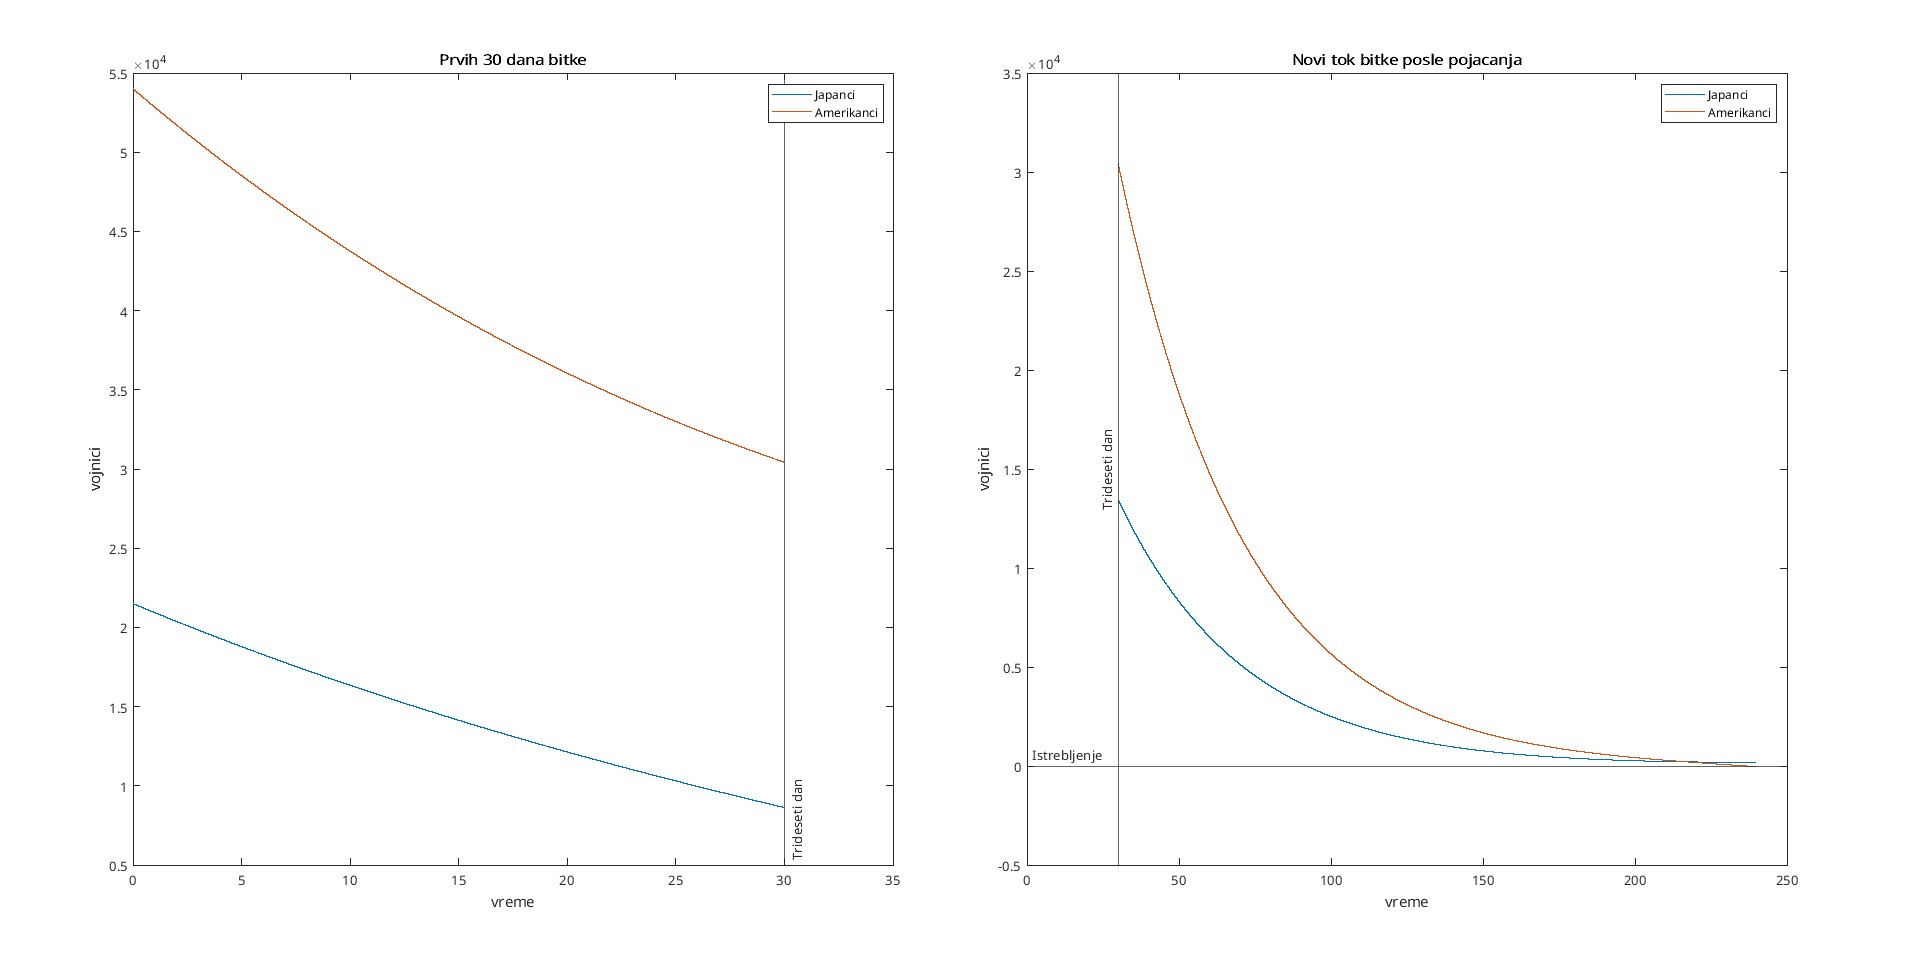
\includegraphics[width=\paperwidth]{img/bitka30.jpg}}
\end{center}

\newpage

\subsection{Kraj bitke za 28 dana}

\vspace{2mm}
\begin{quote}
\textbf{Zadatak 3:}
 Ukoliko je potrebno da se pobeda ostvari za 28 dana, koliko vojnika je
  neophodno da Amerikanci imaju u početku?
\end{quote}

\hspace{5mm}
Pošto će Amerikanci pobediti, onda ce Japanca biti nula posle 28 dana,
tačnije \(J(28) = 0\). Potrebno je pronaći \(A_0\) koje će biti dovoljno
za to. Koristićemo jednačinu (\ref{japanci_cela}), gde je \(t = 28\).

\[
0 = \frac{J_0 \laj - \lambda_A A_0}{2\laj} e^{28 \laj } +
    \frac{J_0 \laj + \lambda_A A_0}{2 \laj } e^{-28 \laj },
\]

Skratimo imenioce i pomnožimo:

\[
  0 = J_0 \laj e^{28 \laj } - \lambda_A A_0 e^{28 \laj} +
  J_0 \laj e^{-28 \laj} + \lambda_A A_0 e^{-28 \laj}
\]

\[
  A_0 \lambda_A (e^{28 \laj} - e^{-28 \laj})
=
  J_0 \laj(e^{28 \laj} + e^{-28 \laj})
\]

\[
  A_0 =
  \frac{J_0 \laj(e^{28 \laj} + e^{-28 \laj})}
  {\lambda_A (e^{28 \laj} - e^{-28 \laj})}
\]
\\
Zamenom konkretnih vrednosti dobije se da početni broj američkih vojnika
jednak \(A_0 = 83040\). \\

\begin{figure}[htbp]
    \center
    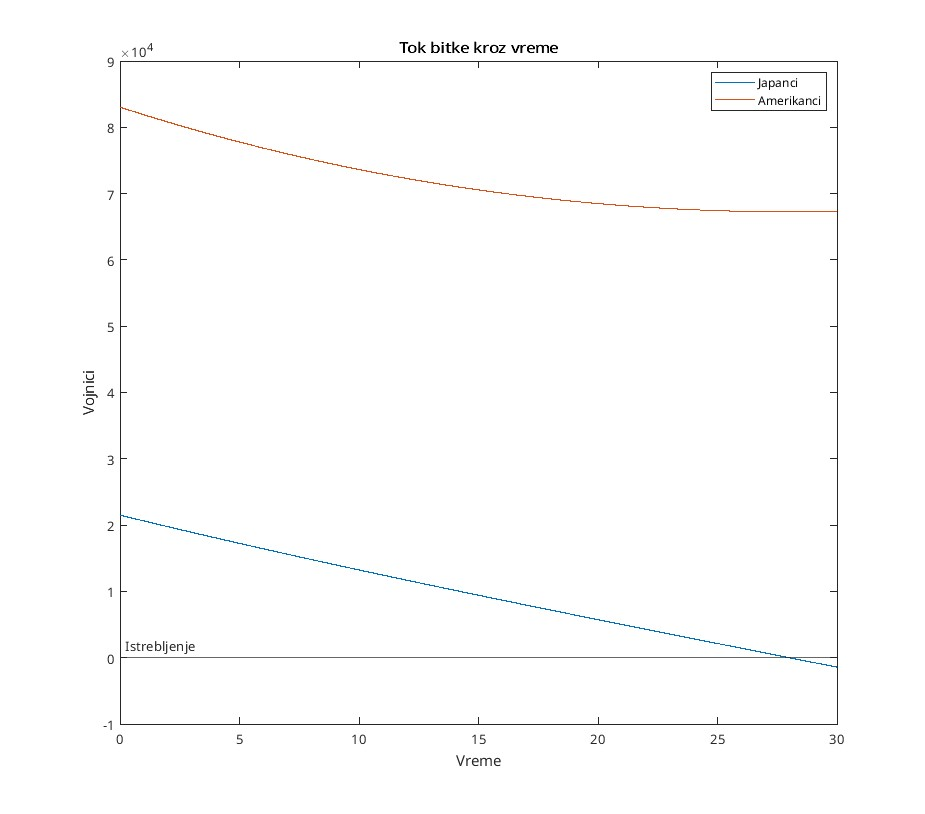
\includegraphics[scale=0.35]{img/bitka28.jpg}
    
\end{figure}


% ------------------------------------------------------------------------------
% Reference and Cited Works
% ------------------------------------------------------------------------------
%\section{Literatura}

\begin{thebibliography}{1}
  \bibitem{wiki}
    \href{https://en.wikipedia.org/wiki/Lanchester's_laws}
         {Lanchester's square law on wikipedia}
  \bibitem{lanchRad}
    Alan Washburn,
    ``Lanchester systems'',
    \url{https://faculty.nps.edu/awashburn/Files/Notes/Lanchester.pdf}
\end{thebibliography}

% ------------------------------------------------------------------------------
\end{document}
